\documentclass[thesis.tex]{subfiles}
\begin{document}
This chapter contains a summary of the finite element method ---
a method for approximating solutions of partial differential equations.
This chapter is mainly included for self-containedness,
a complete mathematical derivation of the theory is well documented in the literature, e.g. \cite{brenner, zienkiewicz1977finite}.
We shall focus on second-order elliptic boundary value problems. For a bounded Lipschitz domain $\Omega \subset \R^n$ the 
general boundary value problem with Dirichlet boundary conditions is solving $u$ from
\begin{equation}
  \label{eq:elliptic}
  \begin{alignedat}{2}
    -\nabla \cdot {\left(\mathbf{A} \nabla u\right)} + \v{b} \cdot \nabla u + c &= &f \quad  &\text {in } \Omega,  \\
  u  &=& 0 \quad &\text{on } \partial\Omega.
  \end{alignedat}
\end{equation}
The theory works equally well for other boundary conditions like Neumann, or Mixed; but we omit
these types for ease of presentation and calculations. Under mild conditions on $\mathbf{A},\v{b}, c$ 
and $f$ we can approximate the solution $u$ of this problem using the finite element method.

\section{Weak formulation}
The first step is translating the boundary value problem \eqref{eq:elliptic} into a \emph{weak formulation}.  
That is, we define a space $V$ of test functions and consider the problem of finding $u$ such that \eqref{eq:elliptic} holds 
in a distributional sense. Suppose that $u$ solves \eqref{eq:elliptic} with $\mathbf{A}, \v{b}, c, f$ sufficiently smooth functions, then for $v \in V$ --- which we will define later on--- we calculate
\begin{align*}
  \ip{f,v}_{\O} = &\ip{-\nabla \cdot {\left(\mathbf{A} \nabla u\right)} + \v{b} \cdot \nabla u + c, v}_{\O} \\
  = &\int_\Omega \left( -\nabla \cdot {\left(\mathbf{A}(x) \nabla u(x)\right)}\right)v(x) + \left(\v{b}(x) \cdot \nabla u(x)\right)v(x) + c(x) v(x) \, \dif x\\
  = &\int_{\partial \Omega} -\left(\mathbf{A}(x) \nabla u(x) \cdot n\right)v(x) \, \dif x \\
  &+ \int_{\Omega} \left( \mathbf{A}(x) \nabla u(x)\right) \cdot \nabla v(x) + \left(\v{b}(x) \cdot \nabla u(x)\right)v(x) + c(x) v(x) \, \dif x.
\end{align*}
Where the third equality follows from the Divergence theorem, see \ref{thm:divergence}. We write $\ip{\cdot, \cdot}_{\w}$ to mean
the standard --- possibly vector-valued --- $L^2(\w)$-inner product on any domain~$\w$. Suppose that all test functions $v$ vanish on the boundary $\partial \Omega$, then the boundary integral disappears and the above simplifies to
\begin{equation}
  \label{eq:ellipticweak}
  F(v) := \ip{f,v}_\O = \ip{\mathbf{A} \nabla u, \nabla v}_\O + \ip{\v{b} \cdot \nabla u + cu, v}_\O=: a(u,v).
\end{equation}

A weak solution of \eqref{eq:elliptic} is a function $u$ that solves the above equation for all $v \in V$.
It turns out that under some conditions there is a unique weak solution $u$. To see this
we must formalise the previous calculations. First we tackle the definition of $V$.

The weak formulation uses the $L^2(\Omega)$-inner product, so we naturally require~$V~\subset~L^2(\Omega)$.
All the partial derivatives of $v$ are taken in a distributive sense.
For these to be correctly defined we need that $v$ is at least weakly differentiable.
By combining both requirements we deduce that $V$ should lie in the suitable space 
$W_2^1(\Omega) = H^1(\Omega)$ (conveniently this is a Hilbert space).
We must check that the calculations, in particular the Divergence theorem, are still valid for $v \in H^1(\Omega)$;
of course this is the case, cf. \cite[Ch. 5]{brenner}.
Formalizing the vanishing boundary requirement can be done using the trace operator $T$\footnote{Here we need that $\Omega$ has a Lipschitz boundary, cf. \cite[Ch. 1.6]{brenner}.},
i.e. we should have $v \in H^1(\Omega)$ such that $\|Tv\|_{L^2(\partial \Omega)} = 0$. All together this yields
\[
  V := \set{v \in H^1(\Omega): v|_{\partial \Omega} = 0} = H_0^1(\Omega).
\]

The Lax-Milgram theorem can be used to show that certain weak formulations have a unique solution.
A proof of this theorem can be found in many books, e.g.~\cite[\S2]{brenner}.
\begin{thm}[Lax-Milgram]
  \label{thm:lax}
  Given a Hilbert space $(V, \ip{\cdot, \cdot})$ and a bilinear form $a(\cdot,\cdot)$ on $V$ which is
  \begin{alignat*}{3}
    \text{Continuous:} \quad & \exists C < \infty \quad & \text{s.t.} \quad & \abs{a(v,w)} \leq C \|v\|\|w\| \quad \forall v,w \in V; \\
    \text{Coercive:}   \quad & \exists \alpha > 0 \quad &\text{s.t.} \quad & a(v,v) \geq \alpha \|v\|^2 \quad \forall v \in V.
  \end{alignat*}
  For every continuous linear functional $F \in V'$ there exists a unique $u \in V$ such~that
  \[
    a(u,v) = F(v) \quad \forall v\in V.
  \]
\end{thm}

Before we can apply  Lax-Milgram to our weak formulation \eqref{eq:ellipticweak} we need restrictions on the parameters $\mathbf{A}, \v{b}, c$ and $f$. We assume that:
\begin{enumerate}[label=(\alph*)]
  \item $\mathbf{A}(x) = (a_{ij}(x))_{1 \leq i,j \leq n}$ is symmetric, $a_{ij} = a_{ji}$, with $a_{ij} \in L^{\infty}(\Omega)$. Furthermore, we suppose that the matrix is uniformly elliptic, i.e. there is a positive constant $\alpha$ such that 
\[
  \zeta \cdot (\mathbf{A}(x) \zeta) \geq \alpha \|\zeta\|^2 \quad \forall \zeta \in \R^n \quad \text{a.e. in } \Omega;
\]
\item $\v{b}(x) = \left(b_1(x), \dots, b_n(x)\right)^\top$ with $b_i \in L^\infty(\Omega)$ such that the weak divergence vanishes, i.e. $\nabla \cdot \v{b} = 0$ in $\Omega$;
\item $c \in L^\infty(\Omega)$ is non-negative;
\item $f  \in L^2(\Omega)$.
\end{enumerate}
Under these assumptions Lax-Milgram can be applied to the weak formulation \eqref{eq:ellipticweak}. The test space $V = H_0^1(\Omega)$ is
a Hilbert space, the form $a(\cdot, \cdot)$ is bilinear, and the functional~$F$ is linear and continuous by Cauchy-Schwarz:
\[
\abs{F(v)} = \abs{\ip{f,v}_\O} \leq \|f\|_{L^2(\Omega)} \|v\|_{L^2(\Omega)} \leq \|f\|_{L^2(\Omega)} \|v\|_{H^1(\Omega)}.
\]
We are left to check the continuity and coercivity of the bilinear form.
\begin{description}
  \item[Continuity]Using H\"older we find
    \begin{align*}
      \abs{a(v,w)} \leq &\int_\Omega \abs{\sum_{i,j} a_{ij} \pd{v}{x_j}\pd{w}{x_i}  + \sum_i b_i \pd{v}{x_i}w + cvw}\\
                   \leq &\sum_{i,j} \norm{ a_{ij}}_{L^\infty(\Omega)} \norm{ \pd{v}{x_j}}_{L^2(\Omega)} \norm{ \pd{w}{x_i}}_{L^2(\Omega)} + \sum_i \norm{b_i}_{L^\infty(\Omega)} \norm{\pd{v}{x_i}}_{L^2(\Omega)} \norm{w}_{L^2(\Omega)} \\
                   &+ \norm{c}_{L^2(\Omega)} \norm{v}_{L^2(\Omega)} \norm{w}_{L^2(\Omega)} \\
                   \leq &C \|v\|_{H^1(\Omega)} \|w\|_{H^1(\Omega)},
    \end{align*}
    where $C$ is a finite constant because $a_{ij}, b_i, c \in L^\infty(\Omega)$. So $a(\cdot,\cdot)$ is indeed continuous.
  \item[Coercivity] This is where our extra assumptions come into play. Since $\v{b}$ has a vanishing weak divergence, a density argument\footnote{Recall that $C_c^\infty(\Omega)$ is dense in $H_0^1(\Omega)$.} shows that for $v \in H_0^1(\Omega)$ we have
    \[
      \int_\Omega \left(\v{b} \cdot \nabla v\right)v  = \int_\Omega \v{b} \cdot \left({1 \over 2} \nabla v^2\right) = - \int_\Omega \left(\nabla \cdot \v{b} \right) {1 \over 2} v^2 = 0.
    \]
    By non-negativity of $c$ we have $cv^2 \geq 0$ on $\Omega$. 
    The Poincar\'e-Friedrich  inequality --- stated in \S\ref{sec:poincfried} --- provides us with a constant $C_\Omega$ such that $\|v\|_{L^2(\Omega)} \leq C_\Omega \|\nabla v\|_{L^2(\Omega)}$ for $v \in H_0^1(\Omega)$. Combining this with the uniform ellipticity of~$\mathbf{A}$~yields,
    \begin{align*}
      a(v,v) &= \int_\Omega \left(\mathbf{A} \nabla v\right) \cdot \nabla v + \left(\v{b} \cdot \nabla v\right)v + cv^2 \\
      &\geq  \int_\Omega \left(\mathbf{A}(x) \nabla v(x)\right) \cdot \nabla v(x)\, \dif x \\
             &\geq  \int_\Omega \alpha \|\nabla v(x)\|^2\, \dif x = \alpha \|\nabla v\|^2_{L^2(\Omega)}\\
             &\geq \frac{\alpha}{2} \left(\frac{1}{C^2_\Omega} \|v\|^2_{L^2(\Omega)} + \|\nabla v\|^2_{L^2(\Omega)}\right) \geq \beta \|v\|^2_{H^1(\Omega)}.
    \end{align*}
    This shows the coercivity of $a(\cdot, \cdot)$.
\end{description}
Hence we may invoke Lax-Milgram to obtain the desired result, namely that there is a unique $u \in V$ that solves the weak formulation \eqref{eq:ellipticweak}.

We cannot expect to (easily) solve the weak formulation in its current form, since this is still an infinite dimensional problem.
Instead one generally solves the Galerkin approximation problem:
\begin{equation}
  \label{eq:galerk_finite}
  \text{Given a finite-dimensional } \VV \subset V \text{: find $U \in \VV$ s.t. } a(U, v) = F(v) \quad \forall v \in \VV.
\end{equation}
This is a finite dimensional problem, and carefully choosing subspaces $\VV$ can lead to increasing approximation accuracy of $U$ --- 
called the \emph{discrete} solution. Another application of Lax-Milgram applied to $\VV$ shows that this system has a unique solution as well.

\begin{rem}
  We have shown that the weak formulation has a unique solution $u \in H_0^1(\Omega)$. We require more smoothness of $u$ to show that this is also a solution to the original boundary value problem.
\end{rem}

\section{Finite Element Space}
  \label{sec:deffem}
  Construction of subspaces $\VV$ can be done in a systematic way using \emph{finite elements}. 
  The general idea is to split the domain $\Omega$ into elements $K$, each with its own function space.
  The space $\VV$ is then constructed by glueing these pieces together. In this section we will summarize the definitions and results
  presented in \cite[Ch~3]{brenner}.
  \begin{defn} 
    A (unisolvent) finite element is a triplet $(K, \mathcal{P}, \mathcal{N})$ where
    \begin{enumerate}[label=(\alph*)]
      \item $K \subset R^n$ is the \emph{element domain}: a bounded closed set with nonempty interior and piecewise smooth boundary;
    \item $\mathcal{P}$ is the space of \emph{shape functions}: a finite-dimensional space of functions on $K$;
  \item $\mathcal{N} = \set{N_1, \dots, N_k}$ is the set of \emph{nodal variables}: a basis for $\mathcal{P}'$.
    \end{enumerate}
  \end{defn}
  \begin{defn}
    \label{def:dualbasis}
    Let an element $(K, \mathcal{P}, \mathcal{N})$ be given. The basis $\set{\phi_1, \dots, \phi_k}$ of $\mathcal{P}$ dual to $\mathcal{N}$ --- so $N_i(\phi_j) = \delta_{ij}$ --- is called the \emph{nodal basis} of $\mathcal{P}$.
  \end{defn}
  \begin{lem}
    Let $\mathcal{P}$ be a $k$-dimensional vector space with $\mathcal{N} = \set{N_1, \dots, N_k} \subset \mathcal{P}'$.
    The set $\mathcal{N}$ is a basis for $\mathcal{P}'$ if and only if $\mathcal{N}$ determines $\mathcal{P}$, i.e. if $v \in \mathcal{P}$ with $N(v) = 0$ for all $N \in \mathcal{N}$ implies that $v = 0$.
  \end{lem}
  Informally a subspace $\VV$ can now be introduced. Consider a partition $\mathcal{T}$ of the domain~$\Omega$ into finite elements,
  i.e. $\overline{\Omega} = \cup_{K \in \mathcal{T}} K$ where $(K, \mathcal{P}_K, \mathcal{N}_K)$ is a finite element.
  We can simply define $\VV$ to be the space of functions in $V$ that coincide with the shape functions on each element,
  i.e. $v \in \VV$ if $v \in V$ and $v|_{K} \in \mathcal{P}_K$ for all $K \in \mathcal{T}$. 
  Without further conditions on the partition we have no way of giving smoothness  properties for the subspace $\VV$ --- we do not even know if it is correctly defined\footnote{In general, two adjacent elements have a non-finite intersection. 
  Therefore $v \in \VV$ might be incorrectly defined on this intersection in a classical sense.}.
  A piecewise polynomial on $\T$ is in $H^1(\O)$ if and only if it is continuous over all interior edges of $\T$.
  It is therefore reasonable to take a subspace $\VV$ consisting
  of continuous functions.

  In the literature a variety of finite elements are used, each element having its pros and cons. For now we will be using  the \emph{Lagrange element}.
  For a triangle $K$ the lowest order Lagrange element  --- also called linear Lagrange --- is given by the 
  triplet $(K, \mathcal{P}_1(K), \set{N_1, N_2, N_3})$, with $\mathcal{P}_1(K)$ linear polynomials and functionals $N_i(v) = v(z_i)$,
  evaluation in the vertices $z_i$ of K. This element can be generalised to a Lagrange element of order $p$ with shape functions $\mathcal{P}_p(K)$: polynomials of order $p$ on $K$.

  To ensure continuity of the subspace $\VV$ we need more regularity in the partition. In this work  we shall therefore consider subdivisions of the domain into simplices (triangles in $\R^2$, tetrahedra in $\R^3$). Implicitly we therefore also require $\Omega$ to have a polyhedral boundary. Because of the continuity requirement we need the partition to be \emph{conforming} (cf. Figure~\ref{fig:triangulation}).
  \begin{defn}
    A triangulation $\mathcal{T}$ is a conforming partition of the domain $\Omega$ into a finite family of simplices.
    Formally,
    \begin{itemize}
      \item $\overline{\Omega} = \cup_{K \in \mathcal{T}} K$;
      \item $\mathring{K_i} \ne \emptyset, \mathring{K_i} \cap \mathring{K_j} = \emptyset \quad \forall K_i, K_j \in \mathcal{T}, K_i \ne K_j$;
    \item If $F = K_i \cap K_j$ for $K_i \ne K_j$, then $F$ is a common (lower dimensional) face of $K_i$ and~$K_j$.
  \end{itemize}
  \end{defn}
  \begin{figure}
    \centering
    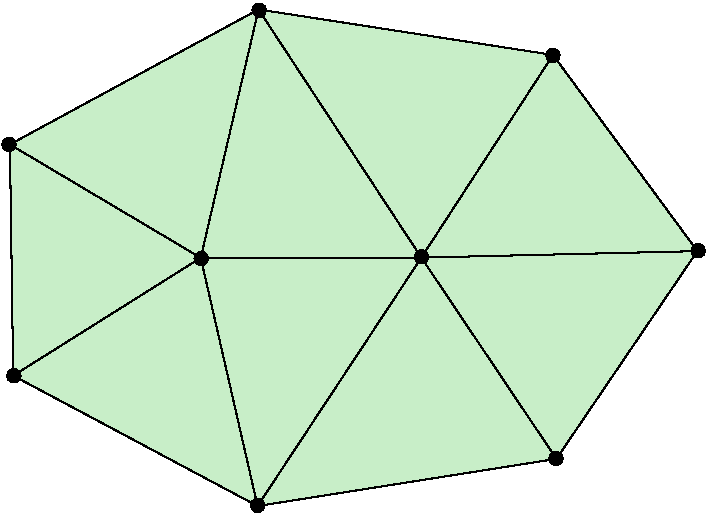
\includegraphics[width=.5\linewidth]{mesh/ex_mesh.pdf}
    \caption{Example of a triangulation for some two-dimensional domain. It has $7$ boundary vertices, and $2$ interior vertices.}
    \label{fig:triangulation}
  \end{figure}

  Consider a triangulation $\T$ and suppose that $\VV$ consists
  of continuous functions $v$ that are linear polynomials when restricted to a triangle $K \in \mathcal{T}$. Formally
  \begin{equation}
    \label{eq:linlagr}
    \VV := \set{v \in C(\OO) : v|_{K} \in \P_1(K), \quad \forall K \in \T}.
  \end{equation}
  Why
  would one look at finite elements $(K, \mathcal{P}, \mathcal{N})$? 
  Instead one could just try to find a basis for this subspace, without ever needing to define finite elements.
  It appears however, that for analysis of the approximation error these finite elements are extremely useful.

  Linear Lagrange elements are an obvious choice for constructing the continuous piecewise linear subspace $\VV$.
  Every function $v \in \VV$ is completely
  determined by its value in the vertices of $\mathcal{T}$, because of continuity and piecewise linearity.
  This precisely coincides with the choice of the local nodal variables. We can therefore lift these local nodal variables to become
  global variables  $\N_\O$ --- a basis for the bigger space $\VV'$. 
  
  As a result we equivalently define $\VV$ to be the span of the global nodal basis with respect to $\N_\O$.   
  For linear Lagrange elements this definition coincides with~\eqref{eq:linlagr}.
  In this construction  we ignored the boundary condition, i.e.  $v \in \VV$ must vanish on the boundary.
   This is easily fixed; we can just consider the (non-trivial)
   nodal variables restricted to $C_0(\OO)'$. In the linear Lagrange case this corresponds to removing nodal variables associated with
   boundary vertices.  

  In short, a basis for the space $\VV'$ can be found by lifting the local nodal variables; where we restrict
  the global variables to the space $C_0(\OO)'$ to ensure the boundary condition.
  For the Galerkin approximation \eqref{eq:galerk_finite} we need more than just continuity; we actually must have $\VV \subset H^1_0(\O)$. This
  weak differentiability  condition is satisfied if one uses Lagrange elements, as summarized in the next lemma (see \cite{brenner} for a proof).
  \begin{lem}
    \label{lem:lin_lagrange}
    Let $\mathcal{T}$ be a triangulation of the domain $\O$, with $\VV$ the finite element space generated
    by using Lagrange elements. Then a function $v \in \VV$ is continuous, weakly differentiable and vanishes on the boundary, i.e.
    \[
      \VV = \set{v \in C(\OO) \cap H_0^1(\O) : v|_{K} \in \P_1(K), \quad \forall K \in \T}.
    \]
  \end{lem}
\section{Interpolant}
\label{sec:apriori}
In the literature the finite element space is frequently defined in terms of the \emph{interpolant} 
(cf. \cite[Ch~3]{brenner}). This interpolant is also an important tool in deriving error bounds. 
  \begin{defn}
    Let $(K, \mathcal{P}, \mathcal{N})$ be a finite element with nodal basis $\set{\phi_1,\dots, \phi_k}$. Then for every function $v$ for which all of the nodal variables $N \in \mathcal{N}$ are defined, the local interpolant is given by
    \[
      I_K v = \sum_{i = 1}^k N_i(v)\phi_i.
    \]
  \end{defn}
  \begin{defn}
    Given a triangulation $\mathcal{T}$ where each $K \in \mathcal{T}$ has an associated 
    finite element triplet $(K, \mathcal{P}, \mathcal{N})$. Then for
    every $v$ that is in the domain of each local interpolant the global interpolant reads as
    \[
      I_{\mathcal{T}} v |_K = I|_K v \quad \forall K \in \mathcal{T}.
    \]
  \end{defn}
  We would like this global interpolant to preserve some regularity. Consider
  linear Lagrange elements again; one easily sees that the global interpolant can be expressed using the global nodal variables, i.e.
    \[
      I_{\mathcal{T}} v = \sum_{i=1}^m N_i(v)\Phi_i \quad \text{ for } \N_\O =\set{N_1, \dots, N_m} \text{ and its global nodal basis } \Phi_1,\dots,\Phi_m.
    \]
    From Lemma~\ref{lem:lin_lagrange} we then see that for $f \in C(\OO)$ one has $I_{\mathcal{T}} f \in C^0(\OO) \cap H_0^1(\O)$. We say
    that the interpolant has \emph{continuity order 0}, and the finite element space $\VV$ is said to be a $C^0$ finite element space.
  \section{Error bounds}
  Given the finite element space $\VV$, one can determine the Galerkin approximation $\eqref{eq:galerk_finite}$. The immediate
  question is of course `what is the quality of the approximation'. Can we find (tight) bounds
  on the approximation error?

  The first such bound is provided by C\'ea's lemma (c.f. \cite[Thm~2.8.1]{brenner}).
  \begin{lem}
    Suppose the assumptions of the Lax-Milgram theorem~\ref{thm:lax} hold. Then for the discrete solution $U \in \VV$ of the
    finite Galerkin approximation \eqref{eq:galerk_finite} we have
    \[
      \| u - U\|_{H^1(\O)} \leq {C \over \alpha} \min_{v \in \VV} \| u - v\|_{H^1(\O)},
    \]
    with $C$ the continuity constant and $\alpha$ the coercivity constant of $a(\cdot, \cdot)$ on $V$.
  \end{lem}
  The above lemma tells us that the finite element solution $U$ is a quasi-best approximation from the subspace $\VV$. We are
  only left to find an element in $v \in \VV$ for which we can bound $\|u - v\|_{H^1(\O)}$. This is where the interpolant comes into play, because $I_{\T}u \in \VV$ if we assume that $u \in C(\OO)$.

  The general idea is to bound $\|v - I_{\mathcal{T}} v\|_{H^1(\O)}$ 
  in terms of local error bounds for each element $K \in \T$.
  First an error bound is derived for a \emph{reference element}~$\hat K$. 
  Then, under certain conditions, this bound can be used to estimate the interpolation error 
  on each of the elements $K \in \T$. The idea of first considering a reference element is often 
  used in finite element analysis and implementation. These extra conditions are formalised by the following definitions.
  \begin{defn}
    A finite element $(K, \P, \N)$ is affine-interpolation equivalent to $(\hat K, \hat \P, \hat \N)$ if there
    exists an affine map $ F(\hat x) = B\hat x + c$ ($B$ non singular) such that for $f = \hat f \circ F$,
    \begin{enumerate}[label=(\roman*)]
      \item $F(K) = \hat K$;
      \item $\P = \{f : \hat f \in \hat \P\}$;
    \item $I_{\hat \N} \hat f = \left( I_{\N} f \right)\circ F$ for all sufficiently smooth $\hat f$.
    \end{enumerate}
  \end{defn}
  \begin{defn}
    Denote $h_K := \text{diam}(K)$ and $p_K := \sup\set{\text{diam}(S): S \text{ ball}, S \subset K}$.
    A~family of finite elements $(K, \mathcal{P}, \mathcal{N})$ is \emph{uniformly shape regular} if 
    \[
      \sup_K h_K/p_K < \infty.
    \]
  \end{defn}
  In words,  $h_K$ is the largest ball containing $K$, whilst $p_K$ is the largest ball inside $K$.
  Shape regularity therefore ensures that triangles do not become \emph{degenerate}.  
  Using the Sobolev inequalities, the Bramble-Hilbert lemma and the Transformation lemma, one
  can proof the following (see \cite[Ch~3]{chen} or \cite{stevenson} for a concise overview).
  \begin{thm}
    Let $(\hat K, \hat \P, \hat \N)$ be a finite element and suppose that $m - n/~2~>~l$,
    \[
      \P_{m-1}(\hat K) \subset \hat \P \subset H^m(\hat K) \quad \text{and} \quad \hat N \subset  C^l(\hat K)'.
    \]
    
    Then there exists a constant $C(\hat K, \hat P, \hat N)$ such that for all $(K, \P, \N)$ affine-interpolation
      equivalent to $(\hat K, \hat P, \hat N)$, and for $0 \leq s \leq m$,
      \[
        \abs{v - I_K v}_{H^s(K)} \leq C \frac{h_K^{m}}{p_K^s} \abs{v}_{H^m(K)} \quad  \forall v \in H^m(\O).
      \]
      If in addition a family $(K, \P, \N)$ is also uniformly shape regular the above is reduced to,
      \[
        \abs{v - I_K v}_{H^s(K)} \leq C h_K^{m -s} \abs{v}_{H^m(K)} \quad \forall v \in H^m(\O).
      \]
  \end{thm}
  This theorem provides us with local error bounds. As a corollary we can now
  give an error bound for the global interpolant.
  \begin{thm}
    \label{thm:apriorio}
    Let $(\mathcal{T})$ be a family of uniformly shape regular triangulations of a domain~$\O \subset \R^n$.
    Suppose that all the finite elements are affine-interpolation equivalent to a reference element $(\hat K, \hat P, \hat N)$,
    then under the conditions of the previous theorem we find for $0 \leq s \leq m$ and $h  := \max_{ K \in \T} h_K$,
    \[
      \left( \sum_{K \in \T} \norm{v - I_K v}^2_{H^s(K)}\right)^{1/2} \leq C h^{m-s} \abs{v}_{H^m(\O)} \quad \forall v \in H^m(\Omega).
    \]
    In case the global interpolant satisfies $I_{\T} C^l(\OO) \subset C^{m-1}(\OO)$, the above left hand side becomes a norm, i.e. 
    \[
      \norm{v - I_{\T}v}_{H^s(\O)} \leq C h^{m-s} \abs{v}_{H^m(\O)} \quad \forall v \in H^m(\Omega).
    \]
  \end{thm}
  Approximate the elliptic problem \eqref{eq:elliptic}  for a family $\T$ of linear Lagrange triangulations and denote $U$
  for respective the discrete solutions.
  Additionally, if the exact $u$ satisfies $u \in H_0^1(\O)\cap H^2(\O)$, then C\'ea's lemma combined with the above theorem tells us that\footnote{
  Here we also used that the global interpolant preserves the Dirichlet boundary condition so that
   $I_{\T} u$ is actually an element of $\VV \subset H_0^1(\O)$.}
  \begin{equation}
    \label{eq:conv}
    \|u - U\|_{H^1(\O)} \leq \frac{C_{cea}}{\alpha} \min_{v \in \VV} \| u - v\|_{H^1(\O)} \leq \frac{C_{cea}}{\alpha} \| u - I_{\T}u \|_{H^1(\O)} \leq \frac{C_{cea}}{\alpha} C  h \abs{u}_{H^2(\O)}.
  \end{equation}
  This provides us with a concrete convergence proof.

  \section{A posteriori error estimation}
  \label{sec:afem}
  This last result \eqref{eq:conv} proves that the approximation error is reduced by solving $U$
  from finite element spaces $\VV$ with decreasing $h$. This so called \emph{a priori} estimator provides an error bound
  using problem specific information, e.g. $u \in H^2$. It does not capture
  any local information; it does not tell \emph{where} the approximation error is substantial. 
  
  In practice one often has $u \not \in H^2$, e.g. if the domain $\O$ has a re-entrant corner, which
  is the case for all non-convex polygon domains. 
  One expects a higher order convergence rate when using higher order (Lagrange) elements.
  Indeed, for $p$ the polynomial degree of the finite element space we obtain the error estimation $\norm{u - U}_{H^1(\O} \leq C h^{p} \abs{u}_{H^{p+1}(\O)}$ from Theorem~\ref{thm:apriorio}. Unfortunately this requires even more smoothness of the exact solution, i.e. $u \in H^{p+1}$. This weakness can --- to some extent ---
  be overcome using an alternative refinement strategy.
  
  Rather than globally reducing $h$, it might be more efficient to consider refinements of~$\T$ with
  the diameter only locally reduced. This is where \emph{a posteriori} error estimators come into play. Given a discrete
  solution $U$, an a posteriori estimator can be used to indicate on which elements $K \in \T$ the error $\|u - U\|_K$ is (relatively) large.

  We follow the terminology used in \cite{stevenson}. For simplicity we restrict ourself to the two-dimensional Poisson problem, i.e. given a polyhedral domain~$\O \subset \R^2$ and $f \in L^2(\O)$:
  \begin{equation}
    \label{eq:poisson}
  \begin{alignedat}{2}
    -\Delta u &=&f \quad &\text {in } \Omega, \\
    u &=& 0 \quad &\text{on } \partial\O.
  \end{alignedat}
\end{equation}
  The bilinear form of the weak formulation is given by $a(v,w) = \ip{\nabla v, \nabla w}_\O$ with
  test and trial space $V = H_0^1(\O)$. This bilinear form
  induces the energy seminorm,
  \[
    \enorm{v}_\O := a(v,v)^{1/2} = \ip{\nabla v, \nabla v}_\O^{1/2} = \abs{v}_{H^1(\O)} \quad \forall v \in V,
  \]
  which is a norm on $V$ thanks to the Poincar\'e-Friedrichs inequality (cf. \S\ref{sec:poincfried}).

  Let $\T$ be a uniformly shape regular triangulation of $\O$. We solve the discrete solution~$U$ from  $\VV(\T)$, the Lagrange finite element space of degree $p$, i.e. 
  \[
    \VV(\T) = \set{ v \in H_0^1(\O ) \cap C(\OO) :  v|_K \in \P_p(K)}.
  \] 

  The classical residual error estimator based on the residual $r \in V'$. In bracket notation for functionals, the latter is defined by
  \begin{align*}
    \ip{r,v} :&= a(u - U, v) = \ip{f,v}_\O - a(U, v).
  \end{align*}
  This is closely related to the approximation error; one easily deduces that
  \begin{equation}
    \label{eq:enormdual}
    \enorm{u - U}_{\O} = \sup_{0\ne v \in V}\frac{a(u - U, v)}{\abs{v}_{H^1(\O)}} = \sup_{0 \ne v \in V}\frac{\ip{r,v}}{\abs{v}_{H^1(\O)}}.
  \end{equation}
  For any $\tilde v \in \VV(\T)$ we can bound the residual using Galerkin orthogonality:
  \begin{align*}
    a(u - U,v) &= a(u - U, v - \tilde v)\\
    &= \sum_{K \in \T} \int_K f(v - \tilde v) + \nabla U \cdot \nabla \left( v - \tilde v\right) \\
    &= \sum_{K \in \T} \int_K (f + \Delta U)(v-\tilde v)+\int_{\partial K} \left(\nabla U \cdot n\right) (v - \tilde v)\\
    &= \sum_{K \in \T} \int_K (f + \Delta U)(v-\tilde v)+\sum_{e \in \E^{int}} \int_e\left \llbracket \nabla U \right \rrbracket  (v - \tilde v)\\
    &\leq \sum_{K \in \T} \| f + \Delta U\|_{K} \| v - \tilde v\|_{K} + \sum_{e \in \E^{int}} \|\llbracket \nabla U \rrbracket \|_{e} \|v - \tilde v\|_{e}.
  \end{align*}
  Here $\llbracket \nabla U \rrbracket$ is the jump of $\nabla U \cdot n$ over an interface in the direction of the unit normal~$n$,
  \[
    \llbracket \nabla U \rrbracket(x) := \lim_{\epsilon \to 0} \nabla U(x + \epsilon n) \cdot n - \nabla U(x - \epsilon n)\cdot n,
  \]
  and~$\E^{int}$~is the set of interior edges of $\T$. The equalities follow from integration by parts and the fact that $v$ vanishes on the boundary edges of $\T$.
  Suppose that we can pick~$\tilde v$ such that $\norm{ v - \tilde v}$ is bound by its seminorm $\abs{v}_{H^1}$. Then combining the above with \eqref{eq:enormdual}
  yields an error estimation for $\enorm{u - U}$ in terms of localized errors on elements and edges.

  We cannot use the interpolants from the previous section to construct $\tilde v$ since they require smoothness of $v$ beyond being in $H_0^1(\O)$.
  The so-called \emph{Scott-Zhang} interpolant~\cite{scott1990finite} does the trick. 
  That is, let  $I_\T : H_0^1(\O) \to \VV(\T)$ be the Scott-Zhang interpolant onto~$\VV(\T)$ as defined in \cite[2.13]{scott1990finite}.
  This local interpolant has the following pleasant local properties
  \[
    \norm{v - I_\tau v}_{K} \leq C h_K \abs{v}_{H^1(\w_K)}, \quad \norm{v - I_\tau v}_{e}\leq C h_{K_e}^{1/2}\abs{v}_{H^1(\w_{K_e})},
  \]
  for all elements $K \in \T$ and edges $e \in \E^{int}$. Here $K_e$ is an element adjacent to $e$, and $\w_K$ is the union of elements touching $K$.
  Inserting $\tilde v = I_\tau v$ into the residual  reveals
  \begin{align*}
    a(u - U, v) \leq& \sum_{K \in \T} \norm{f + \Delta U}_K C h_K  \abs{v}_{H^1(\w_K)} + \sum_{e \in \E^{int}} \norm{\llbracket \nabla U\rrbracket}_e C h_{K_e}^{1/2}\abs{v}_{H^1(\w_{K_e})}\\
     \leq &C \left( \sum_{K \in \T} h_K^2 \norm{f + \Delta U}_{K}^2\right)^{1/2}\left(\sum_{K \in \T}\abs{v}_{H^1(\w_K)}^2\right)^{1/2} \\
    +&C \left(\sum_{e \in \E^{int}}h_K\norm{\llbracket \nabla U \rrbracket}^2_e\right)^{1/2} \left(\sum_{e \in \E^{int}} \abs{v}^2_{H^1(\w_{K_e})} \right)^{1/2}\\
    \leq &  \tilde C \abs{v}_{H^1(\O)} \left(\sum_{K \in \T} h_K^2\norm{f + \Delta U}_K^2 + \sum_{e \in \E^{int}} h_K \norm{\llbracket \nabla U\rrbracket}_e^2 \right)^{1/2},
  \end{align*}
  with the second inequality following from Cauchy-Schwarz for sequences. Together with~\eqref{eq:enormdual} this yields a desired error estimation in terms of
  localized errors:
  \[
    \enorm{u - U}_{\O} \leq \tilde C \left(\sum_{K \in \T}h_K^2\norm{f +\Delta U}_K^2 + \sum_{e \in \E^{int}}h_K\norm{\llbracket U \rrbracket}_e^2 \right)^{1/2}.
  \]
  This gives rise to the following definitions.
  \begin{defn}
    \label{def:clasest}
    For $K \in \T$ and $v \in \VV(\T)$ the residual \emph{error indicator} for $v$ on $K$ reads
    \[
      \eta^2(v, K) := h_K^2 \norm{f + \Delta v}^2_{K} + h_K\norm{\llbracket \nabla v \rrbracket}^2_{\partial K\setminus \partial \O}.
    \]
    The \emph{oscillation term} of $f$ on $K$ is given by
    \[
      \osc^2(f,K) := h_K^2 \norm{f - P_K^r f}^2_{K} \quad \text{ for some } r \geq p-2,
    \]
    with $P_K^r$ the $L^2(K)$-orthogonal projector on polynomials of degree $r$ on $K$.

    For  a subset $\M \subset \T$ the above terms are defined as the sum over $K \in \M$, i.e.
    \[
      \eta^2(v, \M) := \sum_{K \in \M} \eta^2(v, K), \quad \text{and} \quad \osc^2(f, \M) := \sum_{K \in \M} \osc^2(f,K).
    \]
  \end{defn}
  Denote $\T_\star \geq \T$ if $\T_\star$ is a refinement of $\T$. That is, every element in $\T_\star$ is 
  either contained in $\T$ or can be obtained by applying a finite number of bisections to an element in $\T$.
  Write $R_{\T \to \T_\star}$ for the set of refined elements, i.e. $R_{\T \to \T_\star} = \T\setminus \T_\star$.
  To distinguish between finite element solutions, denote $U_\star$ for the Galerkin approximation in $\VV(\T_\star)$. 
  The following theorem holds (see \cite{stevenson} or \cite{cascon2008} for a proof).
  \begin{thm}
    \label{thm:residual_erro}
    There is a constant $C_1$ such that for $\T_\star \geq \T$ we have 
    \[
      \enorm{U_\star - U}^2_{\O} \leq C_1 \eta^2 (U, R_{\T \to \T_\star}) \quad \text{and} \quad \enorm{u - U}^2_{\O} \leq C_1 \eta^2 (U, \T).
    \]

    Similarly, there exists a constant $C_2$ such that
    \[
      \eta^2(U, \T) \leq C_2 \left [\enorm{u - U}^2_{\O} + \osc^2(f, \T) \right].
    \]
  \end{thm}
  Note that the oscillation is dominated by the error estimator, i.e. $\osc^2(f,K) \leq \eta^2(v,K)$. 
  The above lemma therefore shows that the estimator $\eta^2(U, \T)$ provides an upper- and lower bound for the \emph{total error}~$\enorm{u-U}^2_{\O} + \osc^2(f,\T)$.
  That is, the error estimator is proportional to the total error. In practice the $\osc^2(f,\T)$ is often magnitudes smaller 
  than $\eta^2(U,\T)$; if this the case, the estimator $\eta^2(U, \T)$ itself is proportional to the approximation error.

  \section{Adaptive finite element method}
  \label{sec:optimalafem}
  How can one use these local error estimators $\eta(U,\T)$?
  Here we notice that $\eta(U, \T)$ consists of the \emph{known} quantities $f$ and $U$.
  Therefore one can actually compute the estimators  $\eta(U,K)$ to find out \emph{where} the approximation error is big. 
  Instead of globally refining every element, one can just refine the elements for which $\eta(U,\T)$ is large.
  This leads to the very intuitive algorithm, called the \emph{adaptive finite element method}:
  \[
    \texttt{SOLVE} \to \texttt{ESTIMATE} \to \texttt{MARK} \to \texttt{REFINE}.
  \]
  Solve a discrete solution $U$, estimate local errors using $\eta(U, K)$, select a subset of elements for which
  the error is large and refine these elements. Later in \S\ref{sec:afemequil} a more detailed description of this
  method will be given.

  Marking, the selection of triangles to be refined, is  done using D\"orfler marking --- named after its inventor D\"orfler in \cite{dorfler1996convergent}.
  That is, one selects the \emph{minimal} cardinality subset $\M \subset \T$ such that
  $\eta(U, \M) \geq \theta \eta(U, \T)$, for some marking parameter $\theta \in (0,1)$.
  We let \texttt{REFINE} select the smallest refinement  $\T_\star \geq \T$ such that all triangles in $\M$ are bisected. This
  can be accomplished using the \emph{newest vertex bisection} algorithm \cite{traxler1997algorithm, brenner}.

  Write $\set{\T_k, U_k, \M_k}_{k \geq 0}$ for the sequence of results calculated by the adaptive method.
  Using the upper bound from Theorem~\ref{thm:residual_erro}, the D\"orfler marking property, Galerkin' orthogonality and
  the so-called estimator reduction property allows one to proof the following contraction property \cite{dorfler1996convergent,mekchay2005convergence,cascon2008}.
  \begin{thm}
    There exists constants $\gamma > 0$ and $\alpha \in (0,1)$, such that
    \[
      \enorm{u - U_{k+1}}^2_{\O} + \gamma \eta^2 \left(U_{k+1}, \T_{k+1}\right) \leq \alpha\left(\enorm{u - U_k}^2_{\O} + \gamma \eta^2(U_k, \T_k)\right)
    \]
  \end{thm}
  This shows that the \emph{quasi-error} $\enorm{u - U_k}^2_\O + \gamma \eta^2\left(U_k, \T_k\right)$ is reduced at every step.
  Since $\eta^2(U_k,\T_k)$ is proportional to the total error, and $\enorm{u - U_k}$ is a non-increasing sequence, this proves 
  convergence of AFEM.
  One can even prove that this convergence is with the best possible rate. To formalise this we introduce an approximation class.
  \begin{defn}
    \label{def:optimalclas}
    For $s > 0$ define the approximation class $\A^s$ by
    \begin{align*}
      \A^s := \{ u \in H_0^1(\O) :& \Delta u \in L^2(\O),\\
                                  & \abs{u}_{\A^s} := \sup_{N \in \NN} \left(N + 1\right)^s \min_{\set{\T \in \TT : \#\T -\# \T_0 \leq N}} \sqrt{\enorm{u - U_\T}^2_{\O} + \osc^2(f,\T)} < \infty\}.
    \end{align*}
  \end{defn}
  Suppose that $u \in \A^s$. For $\T_N$, the best partition on $N + \#\T_0$ triangles, the total error satisfies $\sqrt{\enorm{u - U_N}_\O^2 + \osc^2(f, \T_N)} \leq  (N+1)^{-s} \abs{u}_{\A^s}$. The number of triangles are in proportion with the number of degrees of freedom; it therefore provides a representative quantity for comparing
  the energy error decay.


  We have the following celebrated optimality theorem. A proof of this theorem as well as an historic overview of contributions that lead to this result
  can be found in \cite{stevenson, cascon2008}. 
  \begin{thm}
    Let $C_1, C_2$ be as in Theorem~\ref{thm:residual_erro}. Ensure that $\theta^2 < \left(C_1(C_2+1)\right)^{-1}$.
    Let $u \in \A^s$ for some $s > 0$, then there is a constant $C$ independent of $u$ such~that
    \[
      \# \T_k - \# \T_0 \leq C \abs{u}^{1/s}_{\A^s} \left( \sqrt{ \enorm{u - U_k}^2_{\O} + \osc^2(\T_k, f)}\right)^{-1/s}.
    \]
  \end{thm}
  In \S\ref{sec:afemequil} we will prove something very similar, but for a different estimator.
  Details of the adaptive finite element method will then become clear.
\end{document}
